\subsection*{\underline{تغییرات نمودار}}

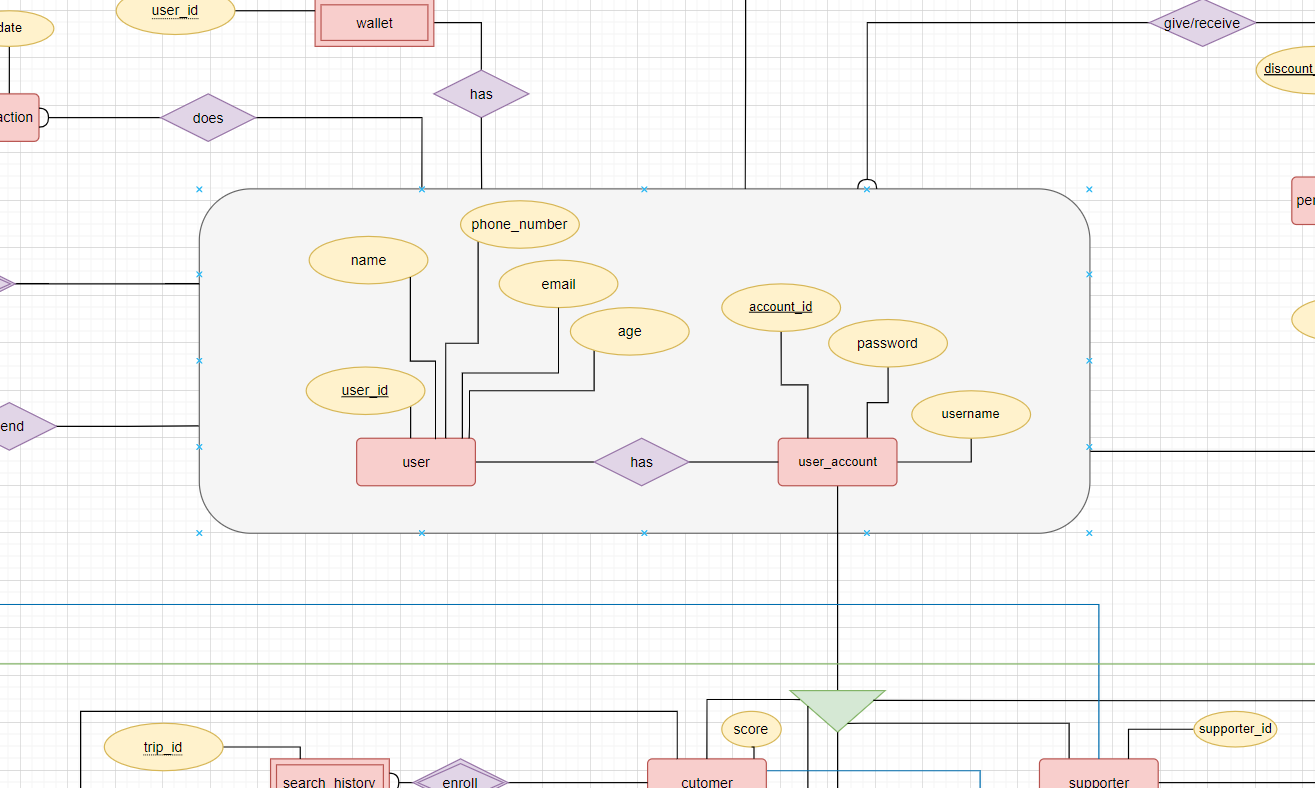
\includegraphics[width=0.5\linewidth]{figs/1-1.png} \
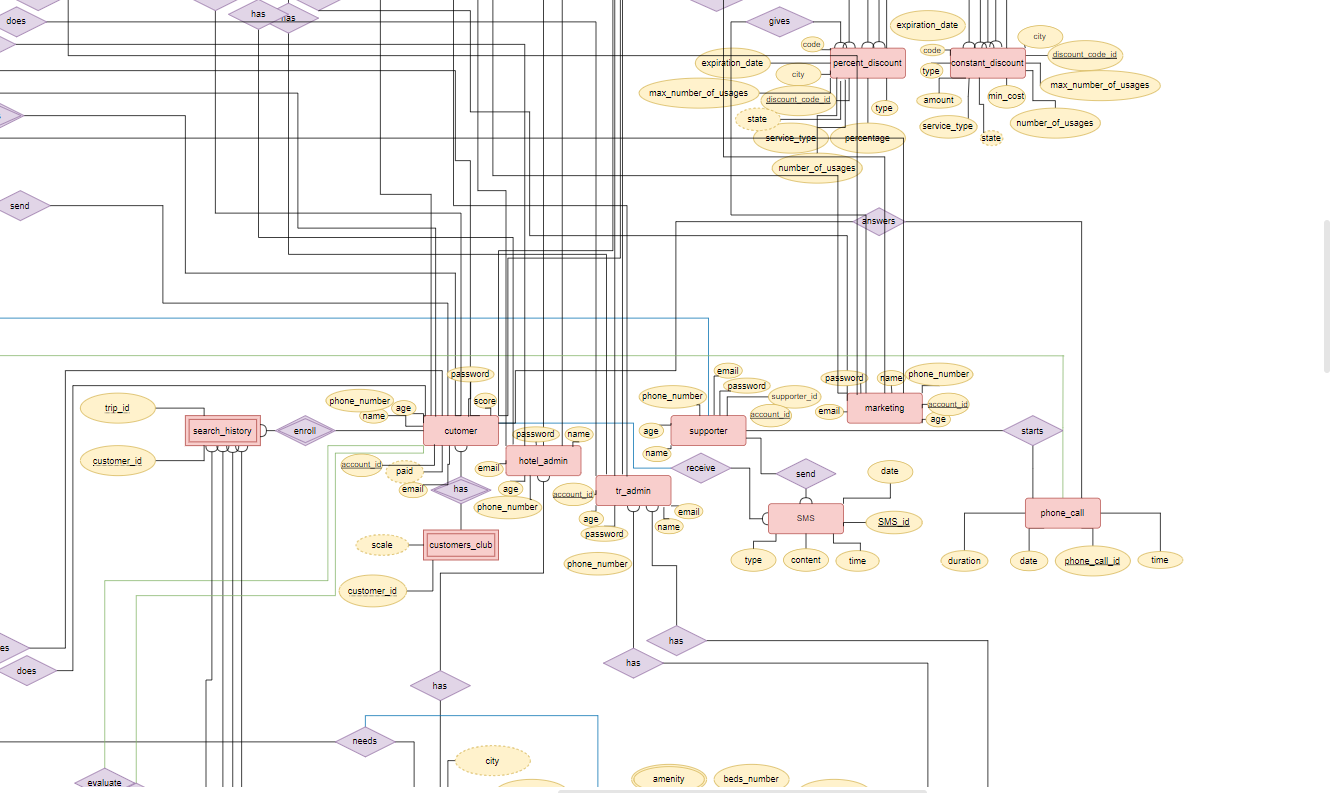
\includegraphics[width=0.5\linewidth]{figs/1-2.png}

اگریگیشن  در SQL وجود ندارد. بنابراین باید شکسته شود. در اینجا تصمیم بر این شد که کاربر و حساب کاربری به دلیل داشن رابطه 1:1 و ویژگی‎های تقریباً مرتبط تبدیل به یک موجودیت شوند و تمام روابطی که به این اگریگیشن متصل است، به userAccount وصل شود.

$\\$

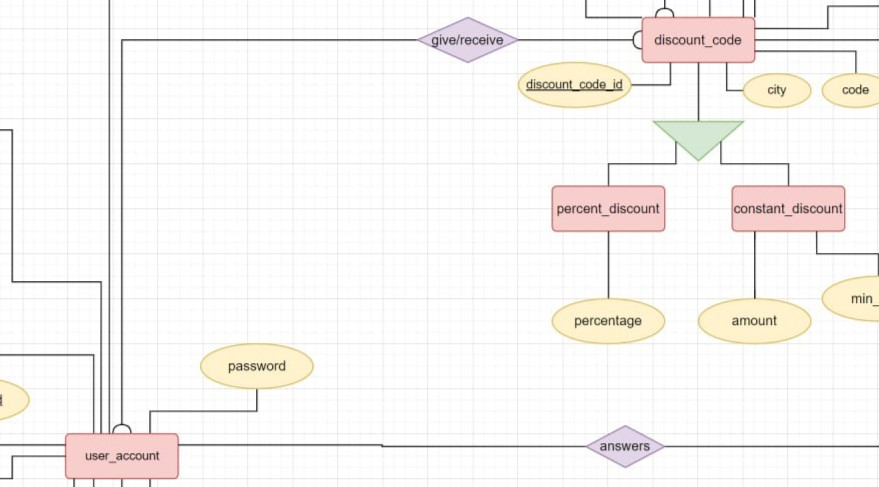
\includegraphics[width=0.5\linewidth]{figs/2-1.jpg} \
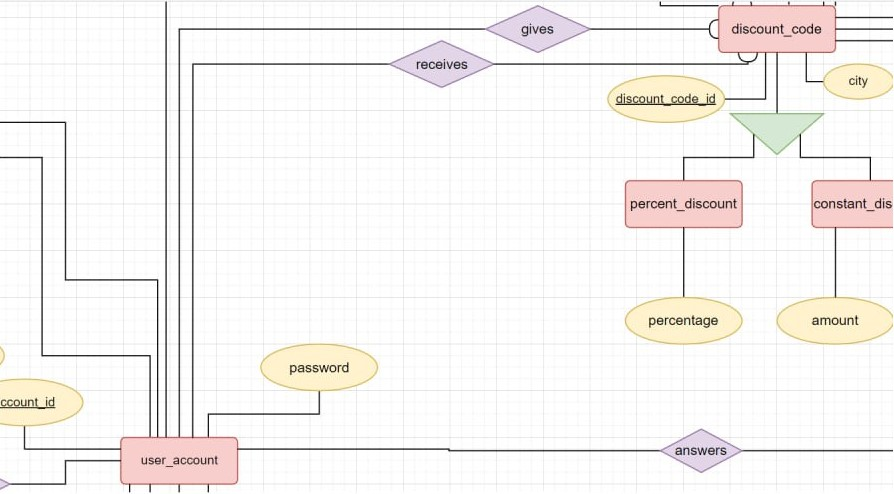
\includegraphics[width=0.5\linewidth]{figs/2-2.jpg}

در گام بعد باید همه روابط manyToMany شکسته شوند. در اینجا رابطه بین discountCode و userAccount باید شکسته شود. برای این کار این رابطه را به دو رابطه تبدیل میکنیم که یکی از آنها مربوط به دریافت‎کننده و دیگری مربوط به اهداکننده کد تخفیف است.

$\\$

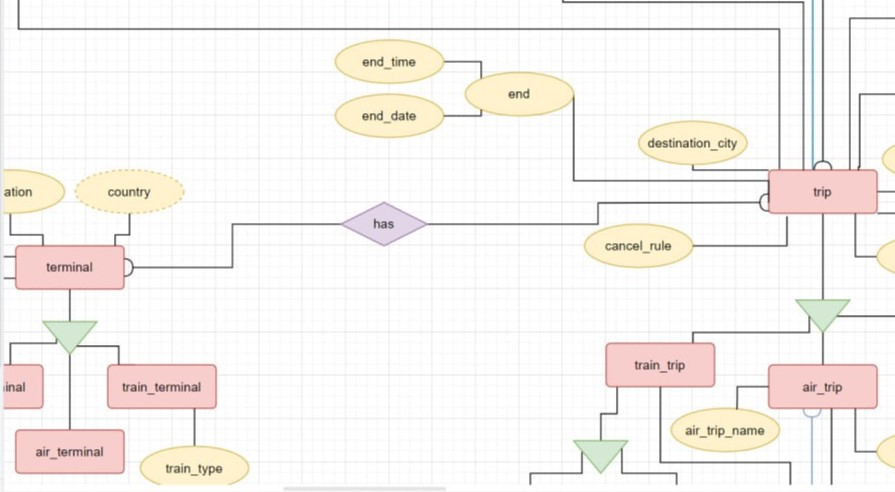
\includegraphics[width=0.5\linewidth]{figs/3-1.jpg} \
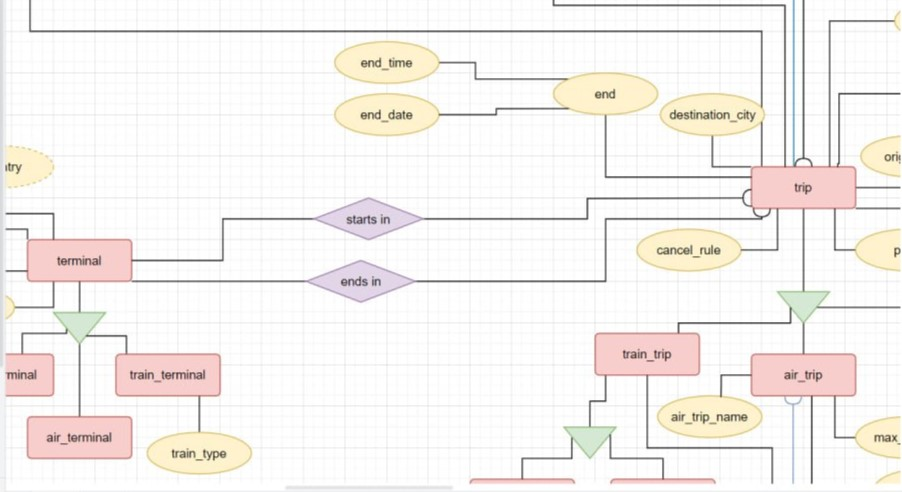
\includegraphics[width=0.5\linewidth]{figs/3-2.jpg}

در اینجا بین trip و terminal رابطه m:n برقرار بود زیرا از هر ترمینال چند سفر انجام می‎شود و هر سفر یک ترمینال مبدا و یک ترمینال مقصد دارد. حالا باید این رابطه را تبدیل به دو رابطه اکنیم که یکی مبدا را مشخص می‎کند و یکی مقصد را.

\pagebreak

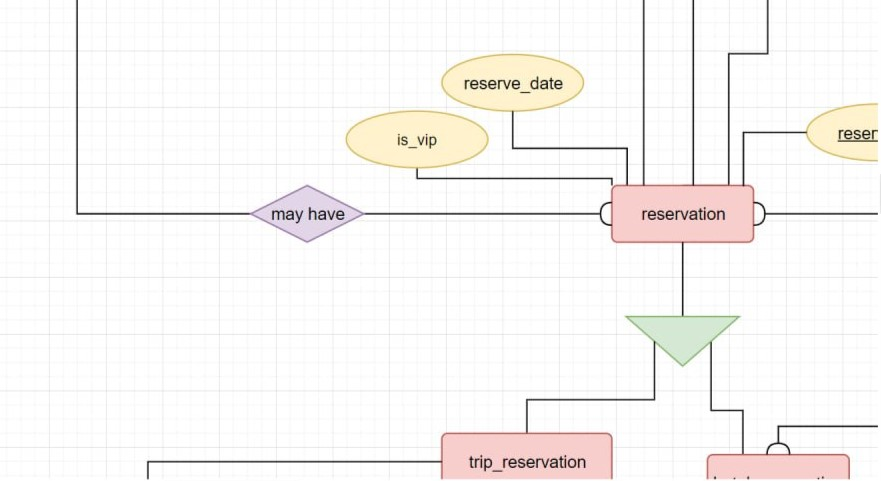
\includegraphics[width=0.5\linewidth]{figs/4-1.jpg} \
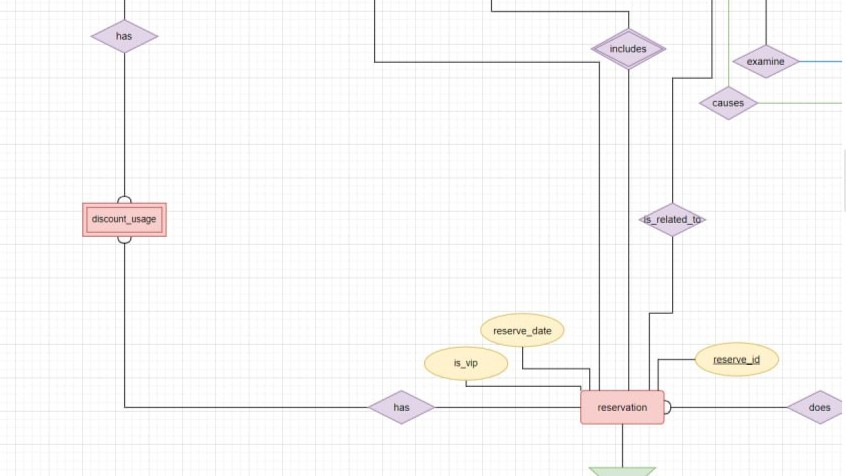
\includegraphics[width=0.5\linewidth]{figs/4-2.jpg}

رابطه بین reservation و discountCode هم m:n بود چون هر کد تخفیف ممکن است بر چند رزرو اعمال شود و هر رزرو چند کد تخفیف داشته باشد. برای حل مشکل می‎توانیم یک موجودیت  ضعیف discountUsage داشته باشیم که کلید خارجی به این دو موجودیت داشته باشد و مشخص کند هر استفاده‎ای از کد تخفیف مربوط به چه کد تخفیفی و برای چه رزروی است.

$\\$

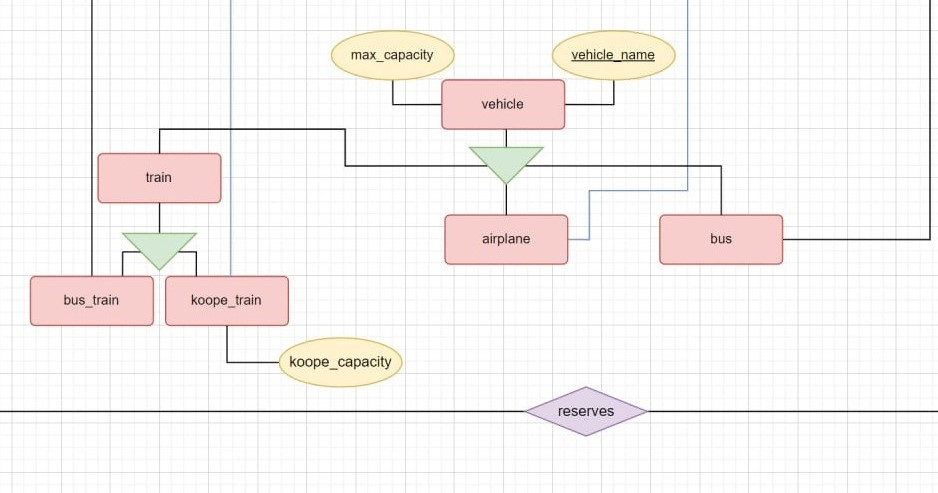
\includegraphics[width=0.5\linewidth]{figs/5-1.jpg} \
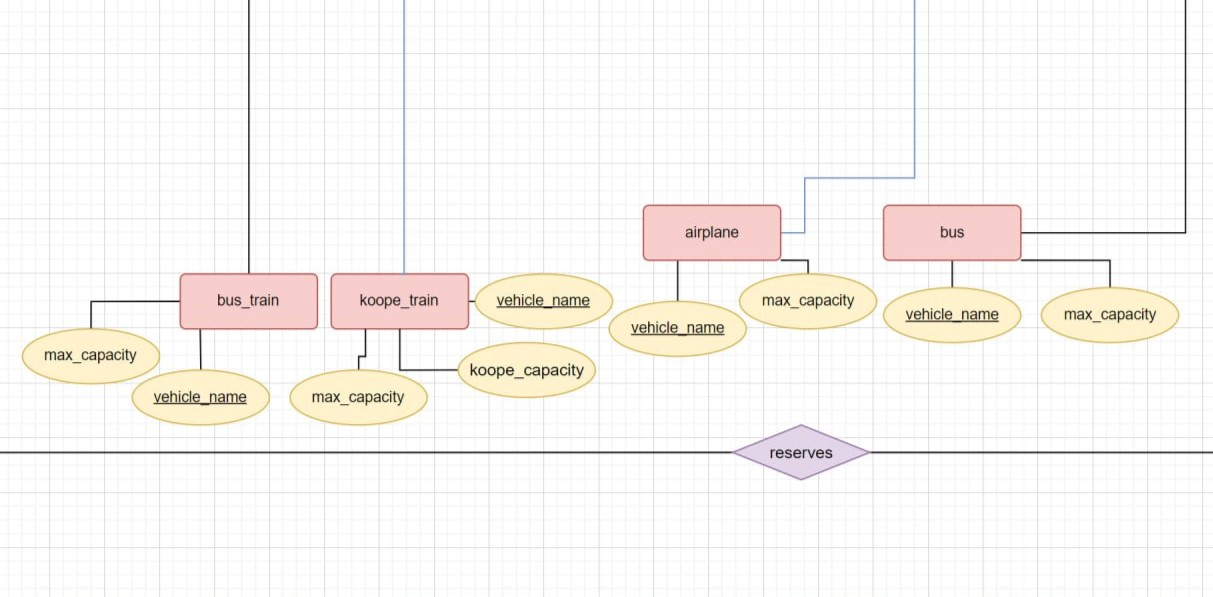
\includegraphics[width=0.5\linewidth]{figs/5-2.jpg}

مورد دیگری که در SQL وجود ندارد ولی در نمودار ما بود، specialization است. برای حل این مشکل موجودیت کلی‎تر را حذف می‎کنیم، و تمام attributeها و روابط آن را به همه موجودیت‎های جزئی آن نسبت می‎دهیم.

$\\$

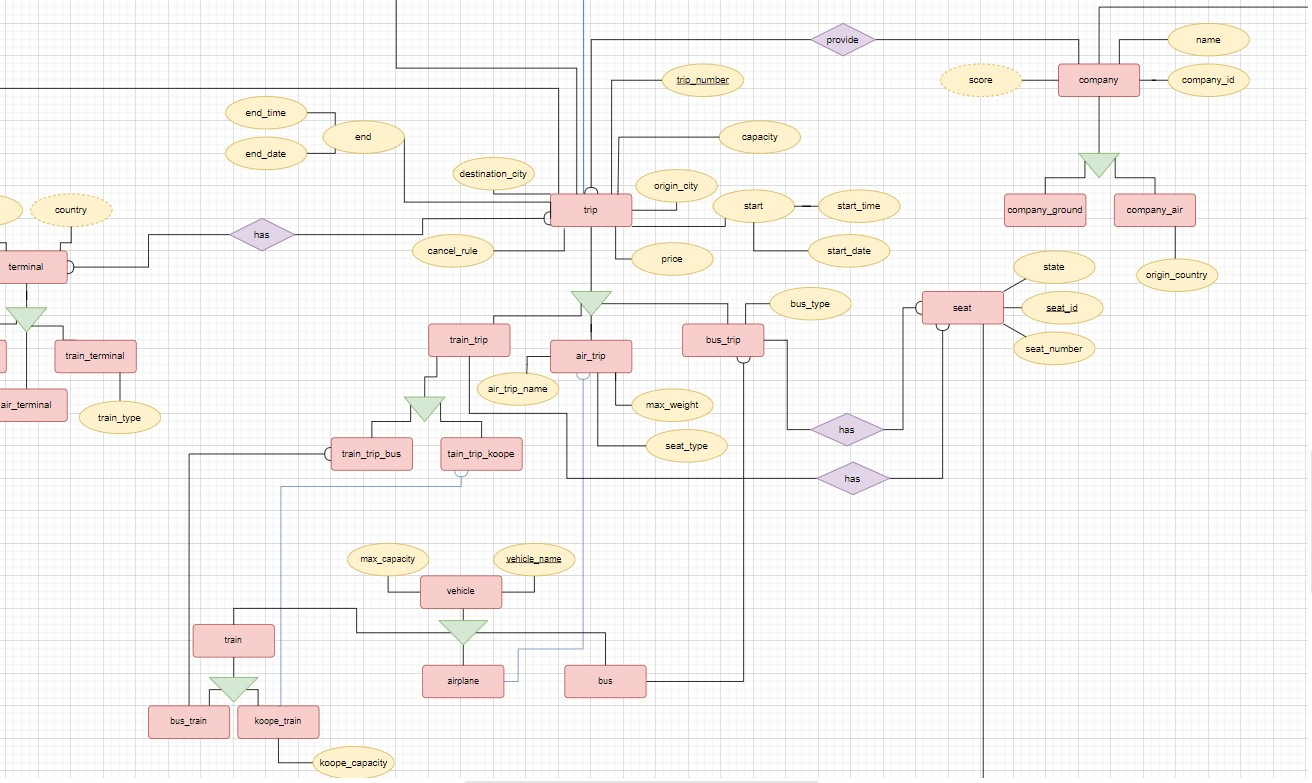
\includegraphics[width=0.5\linewidth]{figs/6-1.jpg} \
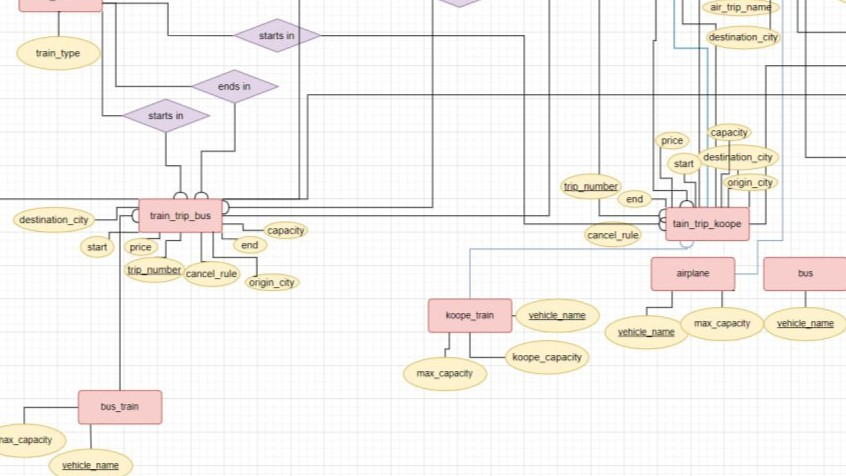
\includegraphics[width=0.5\linewidth]{figs/6-2.jpg}

توضیحات

$\\$

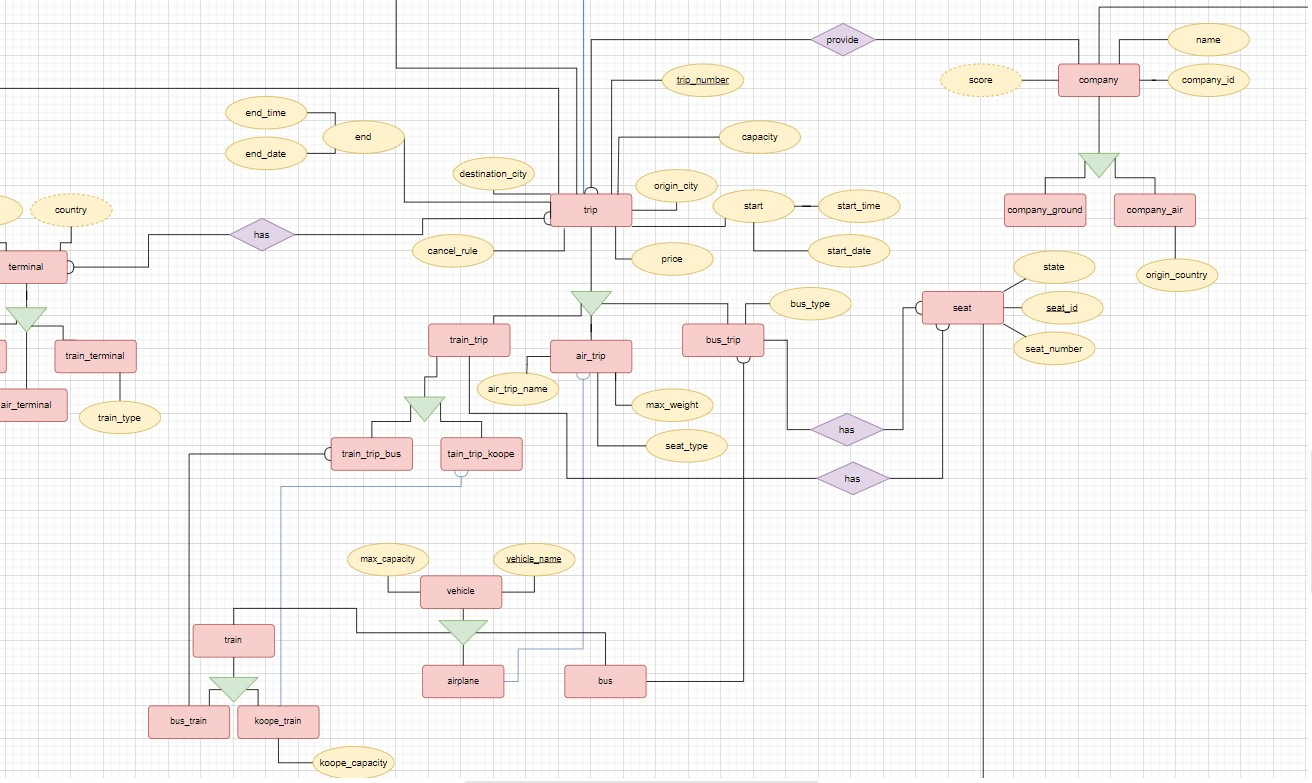
\includegraphics[width=0.5\linewidth]{figs/7-1.jpg} \
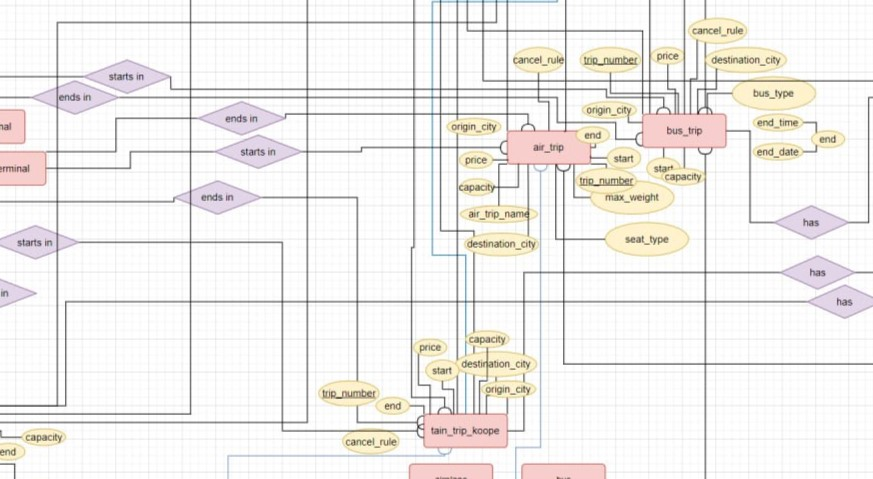
\includegraphics[width=0.5\linewidth]{figs/7-2.jpg} 
توضیحات


$\\$
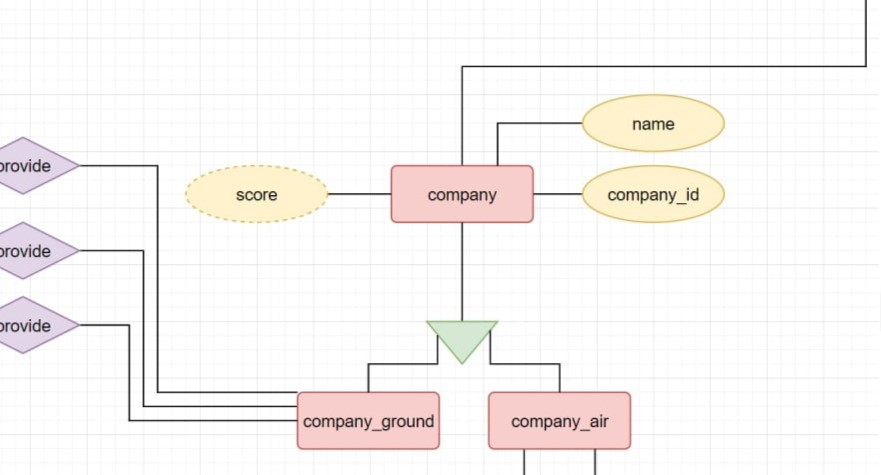
\includegraphics[width=0.5\linewidth]{figs/8-1.jpg} \
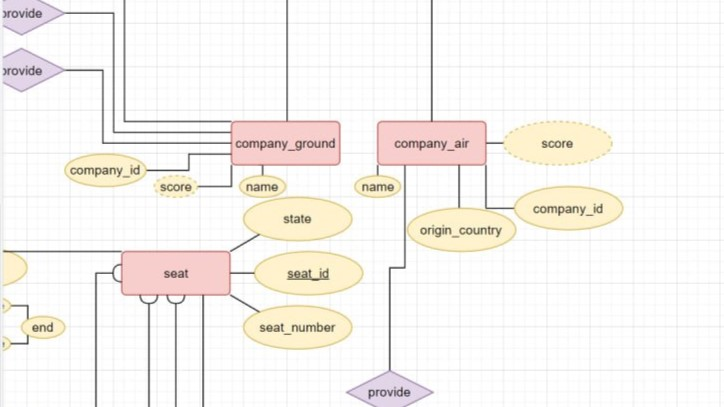
\includegraphics[width=0.5\linewidth]{figs/8-2.jpg} 

توضیحات


$\\$
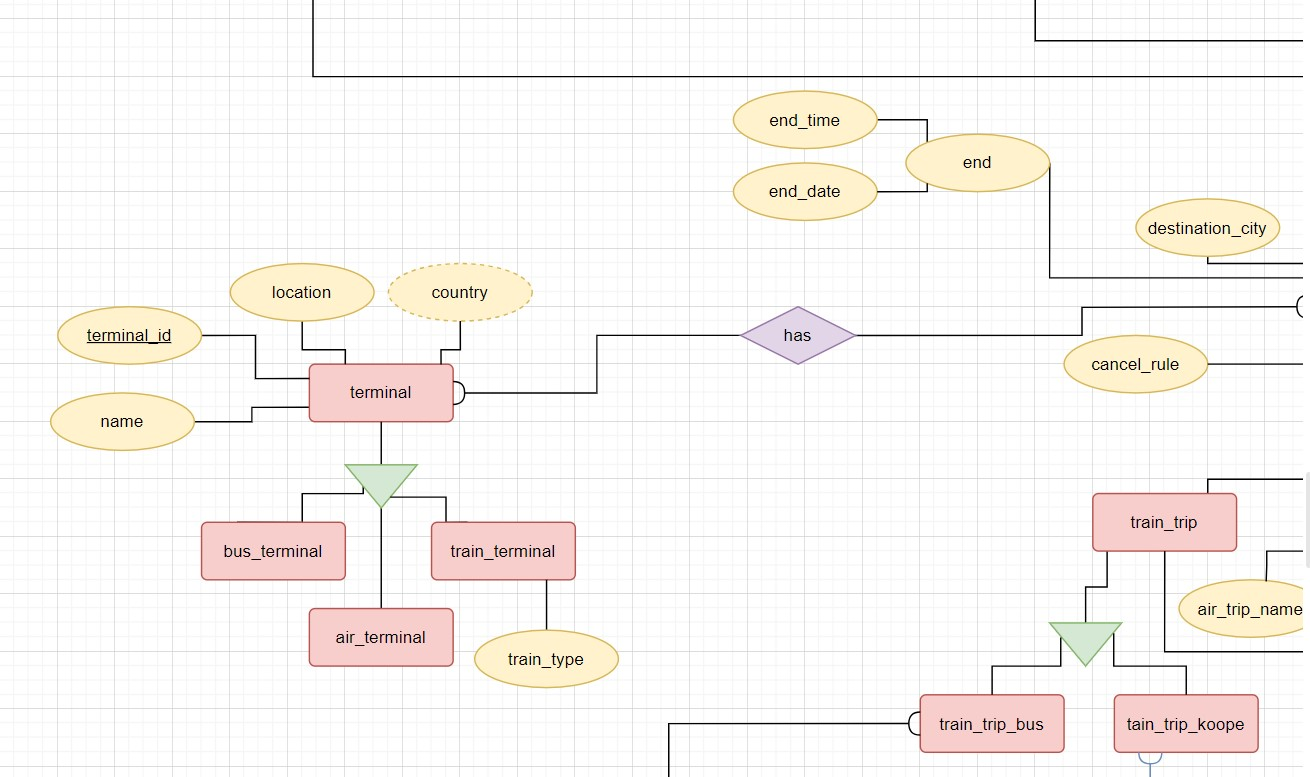
\includegraphics[width=0.5\linewidth]{figs/9-1.jpg} \
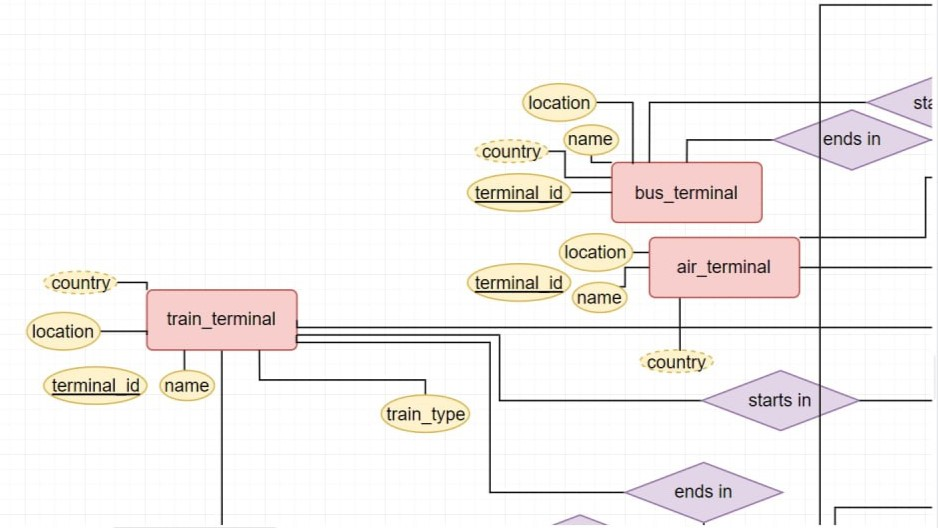
\includegraphics[width=0.5\linewidth]{figs/9-2.jpg} 

توضیحات


$\\ \\$
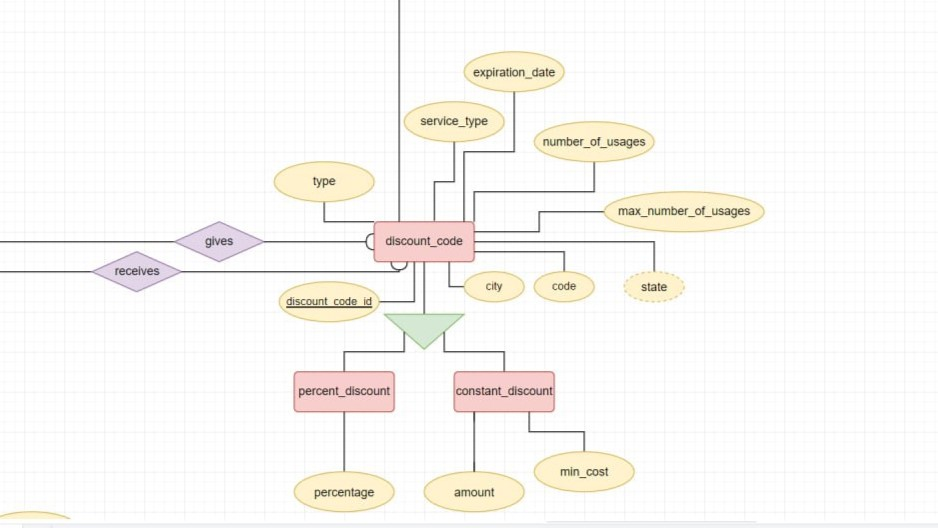
\includegraphics[width=0.5\linewidth]{figs/10-1.jpg} \
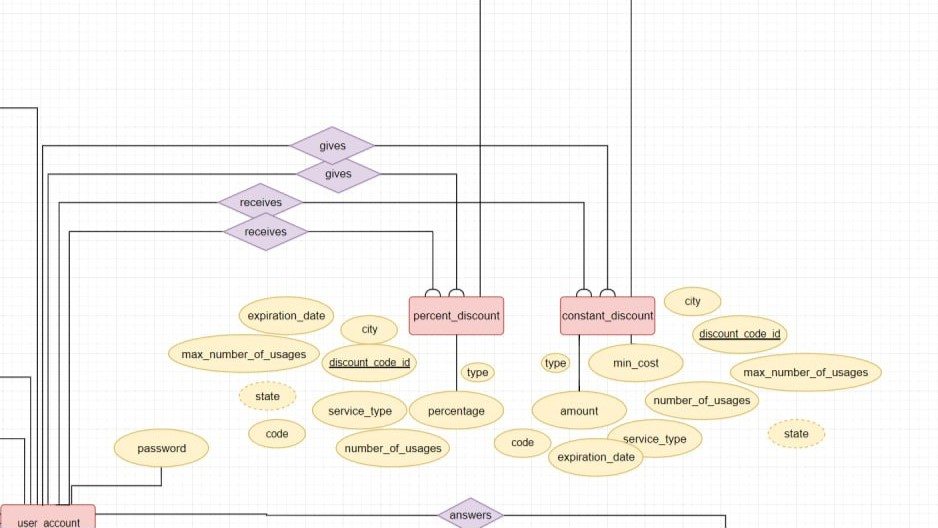
\includegraphics[width=0.5\linewidth]{figs/10-2.jpg} 

توضیحات

$\\$
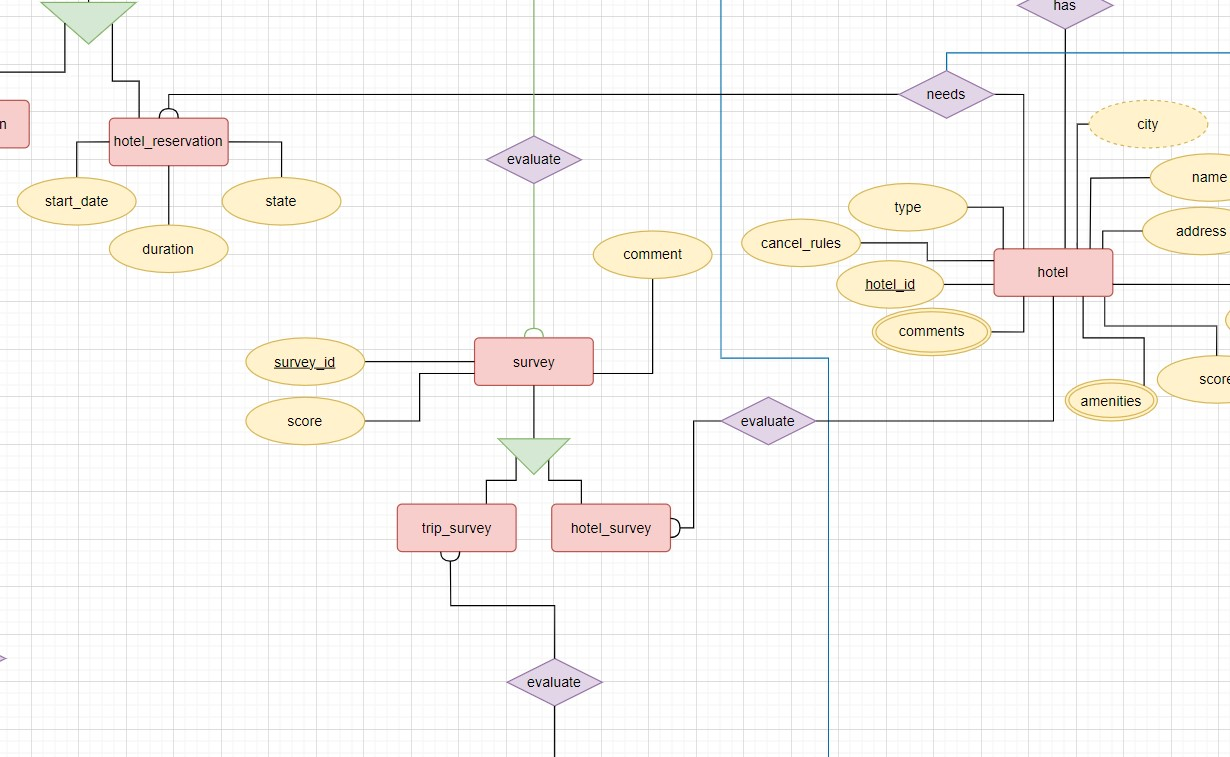
\includegraphics[width=0.5\linewidth]{figs/11-1.jpg} \
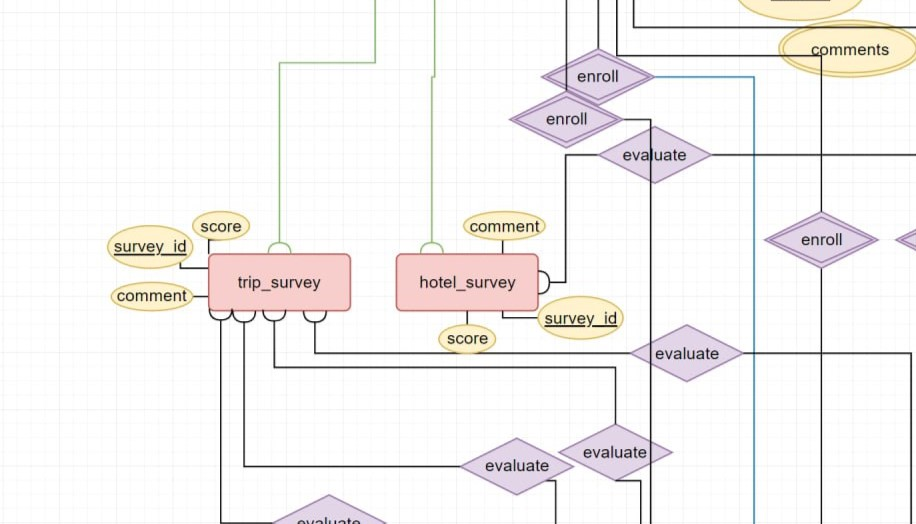
\includegraphics[width=0.5\linewidth]{figs/11-2.jpg} 

توضیحات



$\\$
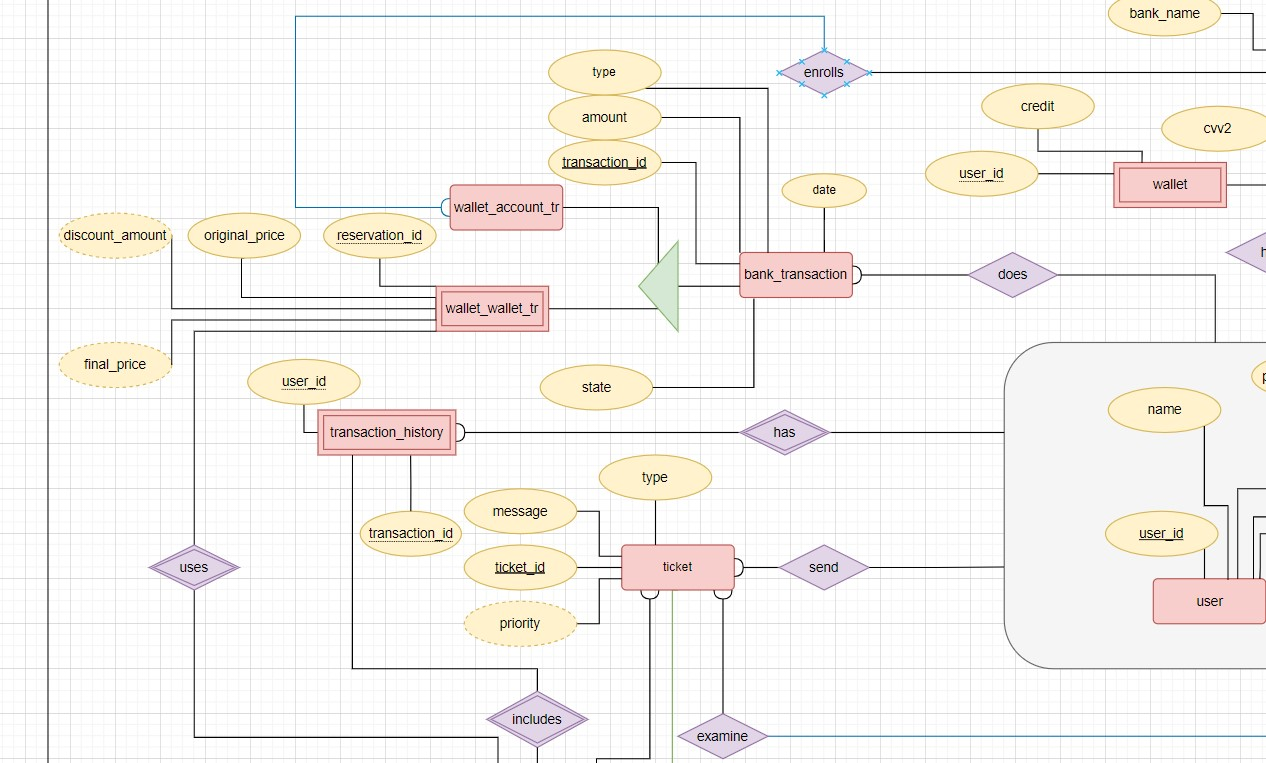
\includegraphics[width=0.5\linewidth]{figs/12-1.jpg} \
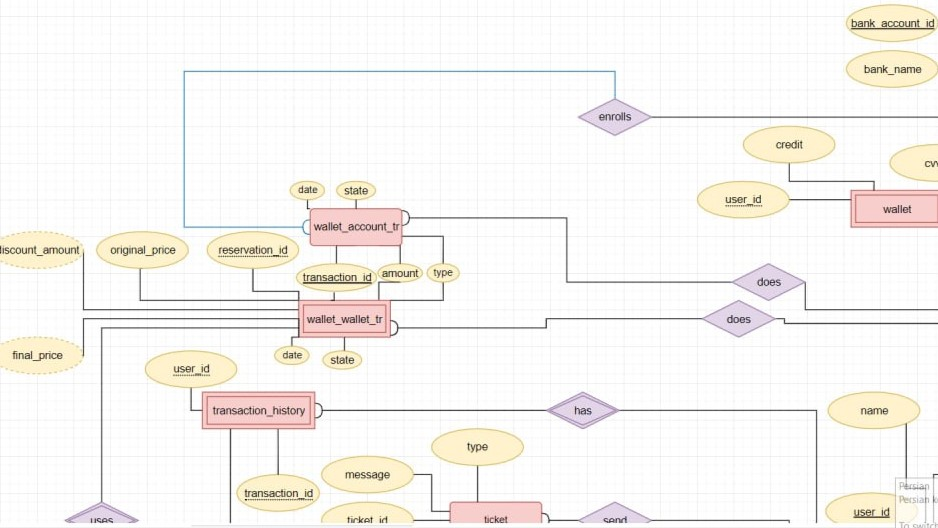
\includegraphics[width=0.5\linewidth]{figs/12-2.jpg} 

توضیحات

$\\$
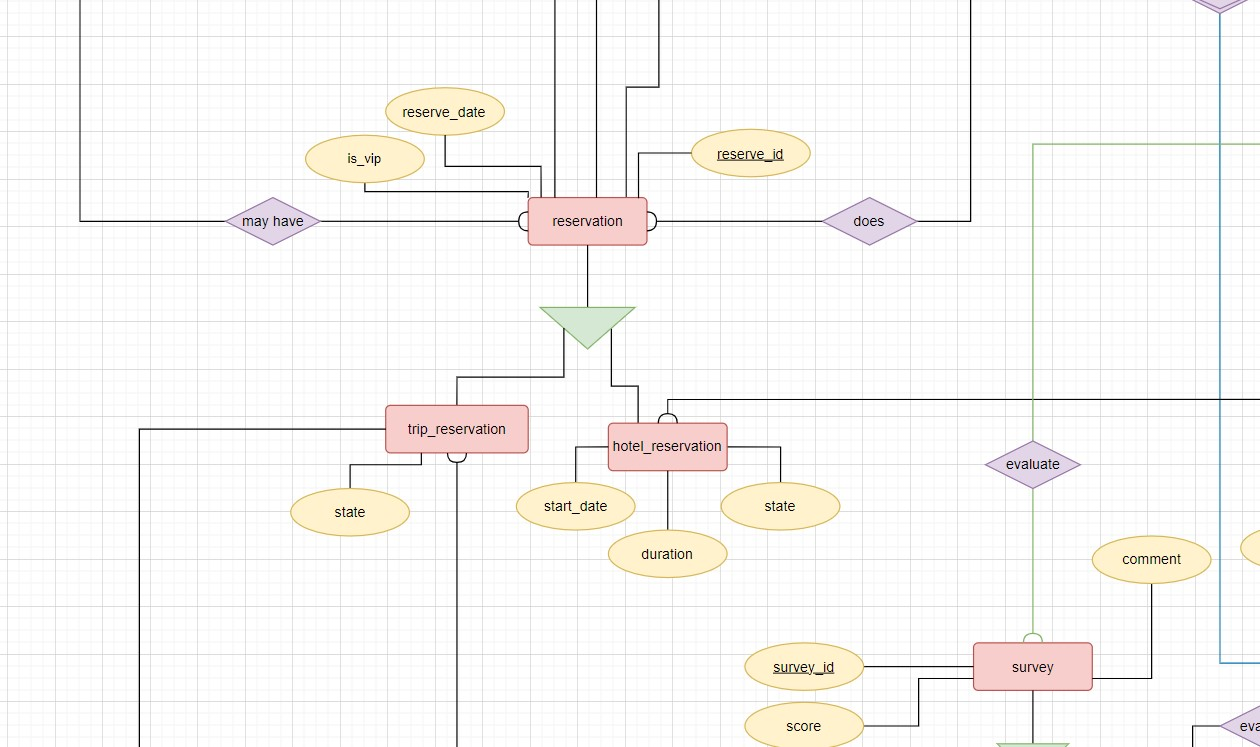
\includegraphics[width=0.5\linewidth]{figs/13-1.jpg} \
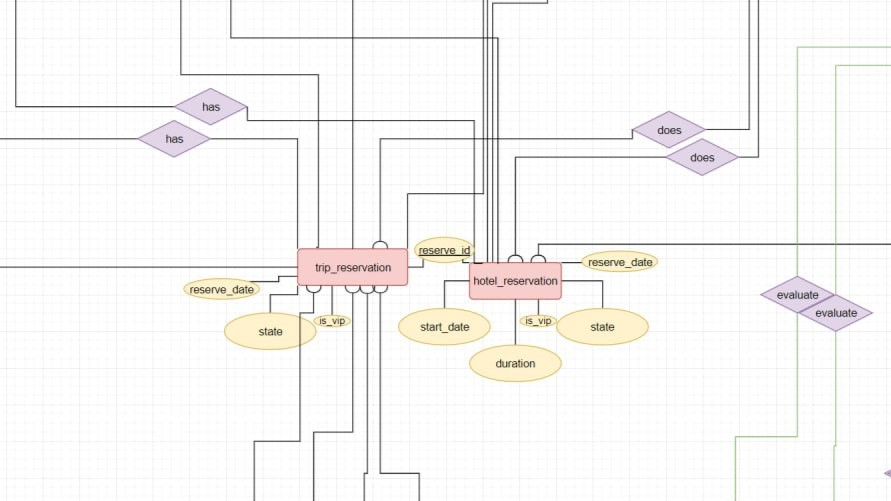
\includegraphics[width=0.5\linewidth]{figs/13-2.jpg} 

توضیحات


